\section{Scelte implementative}
\label{cap:implementation-choices}

\subsection{Codice templatizzato}

Al fine di rendere il codice quanto più generico ed estendibile, molte delle classi e dei metodi scritti
usano i template C++, corrispondenti ai generics in Java.
I nomi ricorrenti dei tipi generici impiegati sono \textit{Label} e \textit{Weight}.
\textit{Label} denota il tipo del nome di un nodo del grafo. È istanziato come \textit{size\_t}, corrispondente a "unsigned long long", occupa almeno 64bit può rappresentare solo valori $\geq 0$.
\textit{Weight} denota il tipo del peso di un arco del grafo. È istanziato come \textit{long}, corrispondente a "signed long int",
occupa almeno 32bit.

\subsection{Rappresentazione del grafo}
\label{sub:graph-representation}

Le due rappresentazioni più comuni per rappresentare un grafo sono \textbf{Matrici di Adiacenza} o \textbf{Liste di Adiacenza}.

Tuttavia in questa implementazione abbiamo scelto di utilizzare una \textbf{"mappa di adiacenza"} affiancata con un set non ordinato per migliorare le complessità temporali di alcune operazioni fondamentali sul grafo, a scapito di un aumento della complessità spaziale. Una prima panoramica della classe è possibile osservarla con il diagramma di classe in figura~\ref{fig:AdjMapGraph Class} dove vengono riportati gli attributi e i metodi offerti dalla classe.

\begin{figure}[h]
	\caption{Diagramma di classe per AdjListGraph}
	\centering
	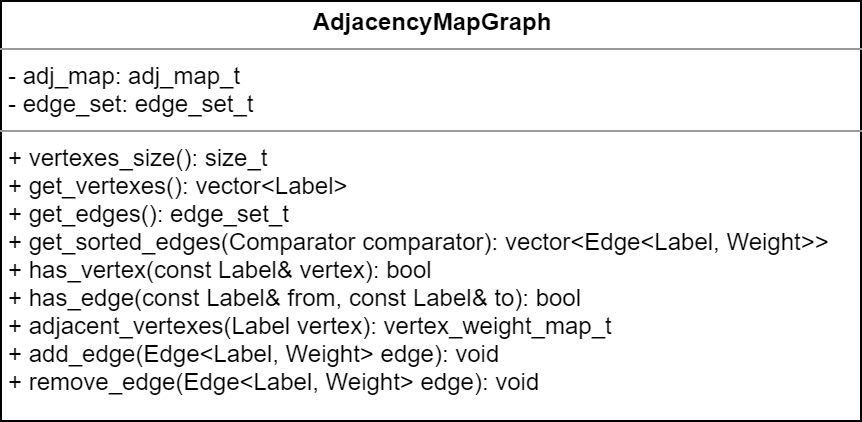
\includegraphics[width=0.7\textwidth]{./images/AdjancencyMapGrapClass.png}
	\label{fig:AdjMapGraph Class}
\end{figure}

Nella figura~\ref{fig:AdjMapGraph Abstract} è riportata la trasformazione di un grafo di esempio nella relativa mappa di adiacenza che abbiamo pensato. Come è possibile notare questa mappa di adiacenza è composta da una prima mappa che elenca tutti i vertici del grafo (adj\_map\_t) e a seguire nel valore di ogni entry viene inserita una nuova mappa (vertex\_weight\_map\_t) che rappresenta gli archi del grafo: vengono elencati dunque tutti i nodi adiacenti al vertice dato con il relativo peso dell'arco. In questo modo è possibile avere tutte le operazioni di inserimento, ricerca, cancellazione e update in tempo costante, a discapito di una complessità spaziale più elevata. 

\begin{figure}[h]
	\caption{Rappresentazione della mappa di adiacenza}
	\centering
	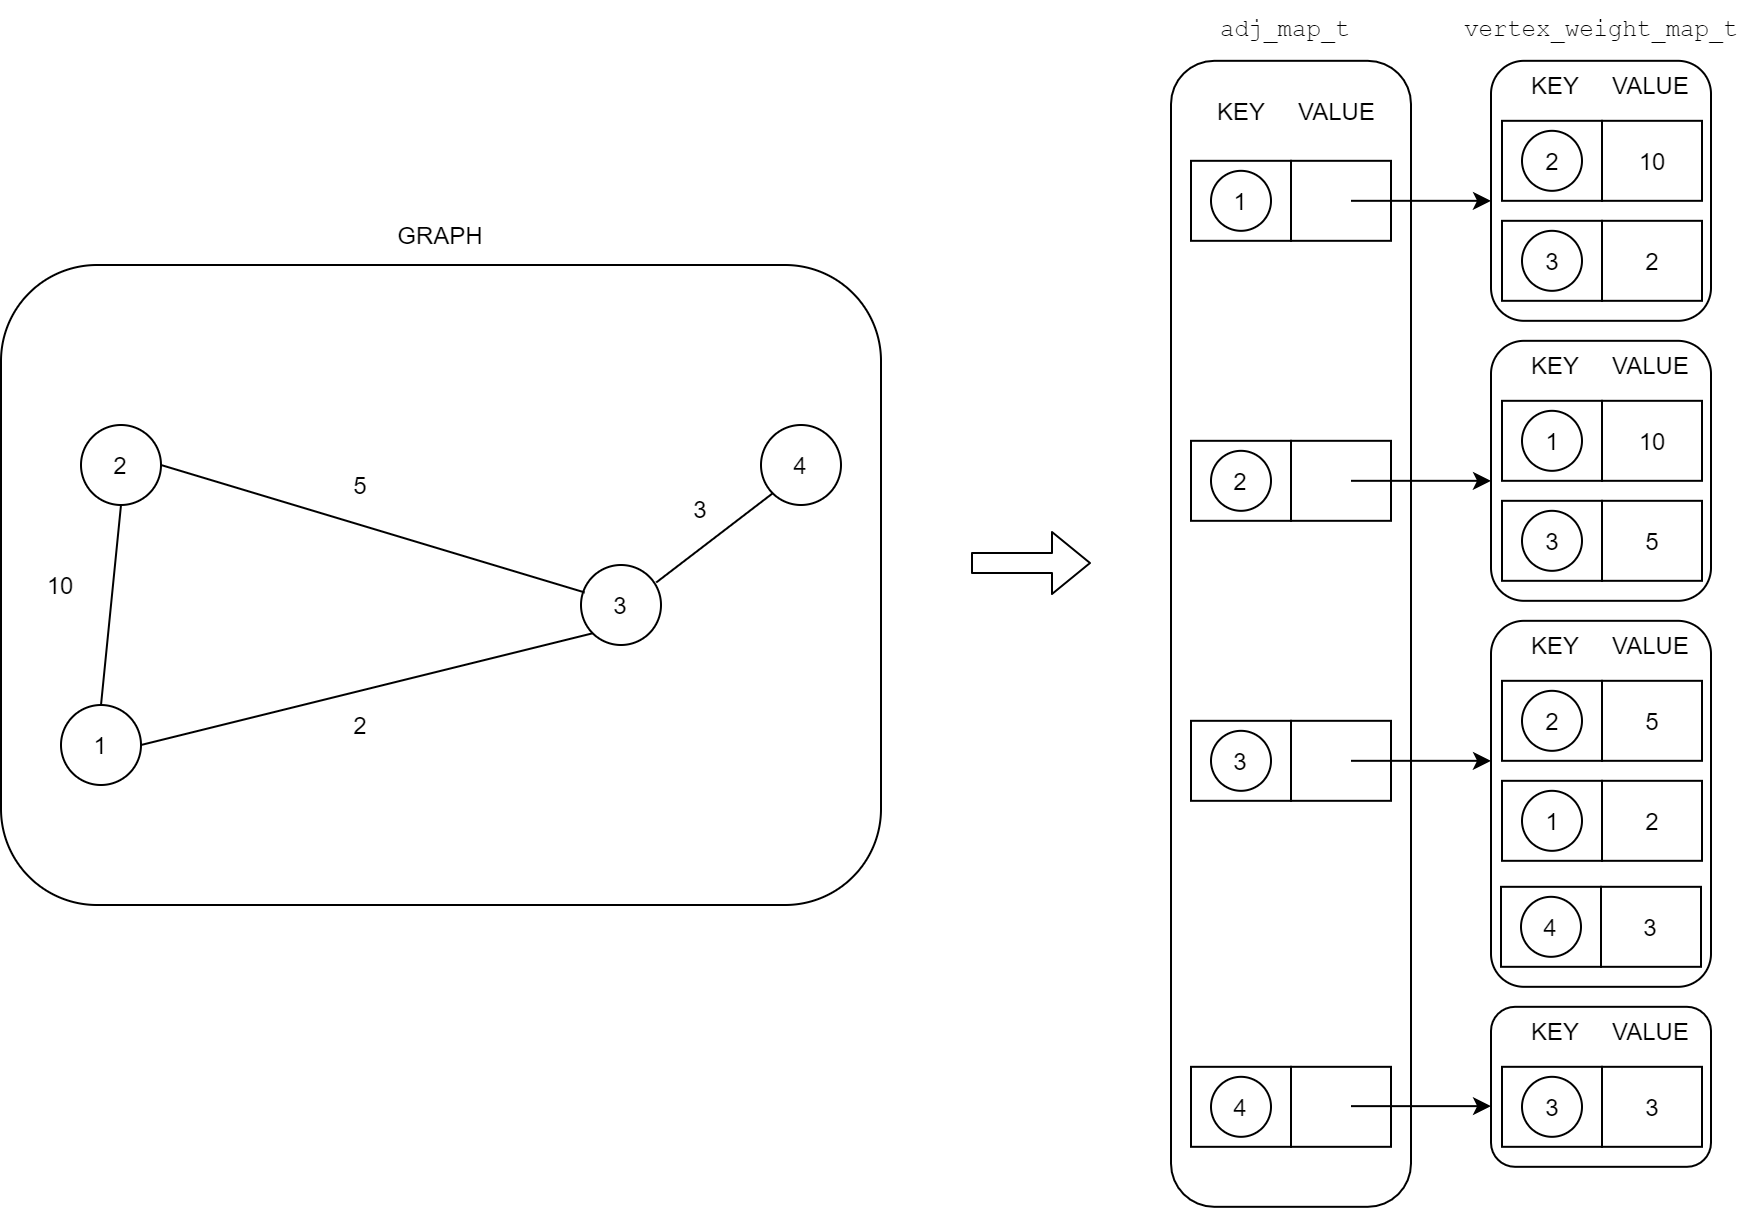
\includegraphics[width=0.7\textwidth]{./images/AdjMapGraphAbstract.png}
	\label{fig:AdjMapGraph Abstract}
\end{figure}

Nonostante la mappa di adiacenza sarebbe già stata sufficiente per salvare tutte le informazioni necessarie alla rappresentazione di un grafo, in alcune operazioni risulta essere lenta. L'esempio di operazione che ci ha spinto ad inserire una nuova struttura dati (unordered\_set in questo caso) è il metodo per ritornare tutti gli archi di un grafo in quanto tale metodo se implementato avendo a disposizione la sola mappa di adiacenza prevederebbe in maniera semplice la scansione dell'intera mappa di adiacenza, con l'inserimento degli archi via via che si incontra un nuovo vertice. Tale semplice implementazione però porterebbe alla creazione di un vettore in cui se sussiste un arco tra un vertice 2 e un vertice 3 (come nell'esempio in figura~\ref{fig:AdjMapGraph Abstract}), al vettore verrebbe aggiunto sia l'arco 2 $\rightarrow$ 3 che 3 $\rightarrow$ 2. \\

Le cose si complicano maggiormente infatti se si restringe la richiesta di non restituire gli archi doppi come abbiamo già osservato. A tale proposito si potrebbe ricercare l'eventuale presenza di tali archi doppi ed eliminarli di conseguenza, ma il tutto richiederebbe maggiori operazioni e dunque un maggior complessità temporale.\\

Per tali ragioni è stato deciso di affiancare alla mappa di adiacenza, un'apposita struttura dati che permettesse di tenere traccia degli archi e di avere tempi di esecuzione costanti per le operazioni di aggiunta, rimozione e ricerca. Così facendo è possibile garantire che l'operazione di restituzione degli archi singoli di un grafo abbia tempo O(m) se si richiede di restituire un vettore, o addirittura O(1) se si richiede la restituzione di un puntatore a tale struttura.
E' stato scelto dunque di utilizzare come struttura dati da affiancare unordered\_set perché oltre ad avere le caratteristiche richieste, se appositamente configurata permette di garantire l'assenza di archi doppi, compresi quelli visti nell'esempio precedente (ossia 2 $\rightarrow$ 3 e 3 $\rightarrow$ 2). Per fare ciò è stato dunque opportunamente configurato l'operatore di uguaglianza e la funzione di hash, in  modo che archi equivalenti abbiamo la stessa funzione di hash e siano riconosciuti come uguali, evitando così l'inserimento di un arco doppio visto che  unordered\_set non prevede elementi doppi al suo interno.\\

Una rappresentazione astratta di tale struttura è possibile visualizzarla nella figura~\ref{fig:edges_set}, dove è possibile notare che se viene richiesto l'inserimento di un arco 3 $\rightarrow$ 2 ove già presente un arco 2 $\rightarrow$ 3 questo non viene inserito da unordered\_set.\\

\begin{figure}[h]
	\caption{Visualizzazione astratta di edges\_set}
	\centering
	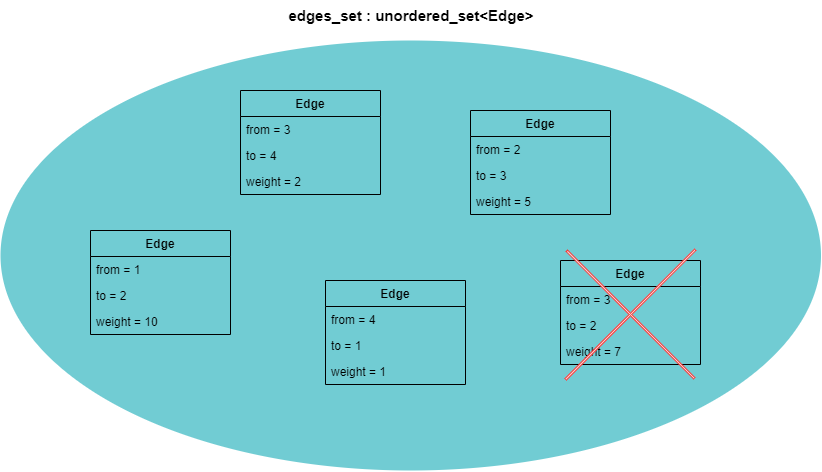
\includegraphics[width=0.7\textwidth]{./images/edges_setAbstract.png}
	\label{fig:edges_set}
\end{figure}

L'ultimo problema non ancora affrontato riguarda la possibilità di inserire un arco doppio tra due nodi uguali (come richiesto da problema), con la differenza che questi 2 archi hanno un peso diverso. Siccome la nostra implementazione non prevede la presenza di tali archi doppi, la funzione add\_eddge() si occupa di verificare l'eventuale presenza di un arco già inserito e di conseguenza i relativi pesi, per andare a modificare il peso qualora il peso del nuovo arco sia inferiore al peso dell'arco precedentemente già inserito. Per fare questo ad ogni aggiunta di un nuovo arco si va a verificare nella lista di adiacenza l'esistenza di un arco per quei due vertici:
\begin{itemize}
	\item \textbf{se l'arco era già stato aggiunto:} si confrontano i due pesi e si aggiorna il peso dell'arco solo nell'eventualità in cui il nuovo peso sia inferiore a quello già presente nella lista di adiacenza. Dopodiché se c'è stato un aggiornamento si aggiorna anche il relativo unordered\_set, eliminando l'arco precedente e si ri-aggiunge l'arco con il nuovo peso. 
	\item \textbf{se l'arco non era già stato inserito:} si inserisce l'arco sia nella lista di adiacenza che nell'unordered\_set.
\end{itemize}

Tutte le operazioni di aggiunta, per come sono implementati unordered\_set e unordered\_map in C++ hanno tempo costante e dunque l'operazione di aggiunta richiede tempo costante.

\subsubsection {Costruzione del Grafo}

\textit{Shared/adjacency\_map\_graph\_factory.h} definisce una funzione di utilità che scorre tutte le righe del file in ingresso, salva gli archi in un vettore temporaneo, e lo trasferisce tramite \textit{move semantics} ad un nuovo oggetto di tipo \textit{AdjacencyMapGraph}. La mappa di adiacenza interpreta il grafo come spiegato nella sezione \ref{sub:graph-representation}.

\subsection{Strutture Dati}

Tutte le strutture dati elencate di seguito sono definite nella cartella \textit{Shared}.
Ove possibile, per la nomenclatura dei metodi abbiamo cercato di seguire lo stesso standard dei container STL di C++.
Inoltre, le strutture dati usate sono sempre preallocate in memoria quando possibile, evitando rehashing e riallocazioni dispendiose. Questo significa che la maggiorparte delle operazioni indicate con \complexity1{} ammortizzato siano in realtà totalmente costanti nella pratica.

\subsubsection{Heap}

\textit{Heap.h} contiene la definizione astratta di una generica Heap.
Gli elementi della Heap sono salvati in un \textit{std::vector}.
Per generalizzare il concetto di MinHeap/MaxHeap, la classe usa un comparatore binario booleano. Se il funtore dato in input alla classe è
\textit{std::greater<>}, la struttura dati avrà la semantica di una Min Heap; viceversa, col comparatore \textit{std::less<>} si avrà la semantica di una Max Heap.

\paragraph{Ottimizzazioni}\mbox{} \\

\noindent Il parametro template \textit{IsAlreadyHeap} è usato per evitare di costruire la Heap se l'utente specifica il container dato in input alla struttura dati rispetta già la proprietà di essere una Heap. Il controllo su questo flag booleano avviene a compile-time. Questa ottimizzazione garantisce un risparmio di tempo pari a \complexityN{}, ed è usata nell'implementazione dell'algoritmo di \textbf{Prim}. \\

\noindent I metodi che ripristinano la prioprietà di Heap (\textit{heapify\_up} e \textit{heapify\_down}) sono definiti in maniera iterative invece che ricorsiva, ottenendo performance migliori a parità di input.

\subsubsection{Binary Heap}

\textit{BinaryHeap.h} contiene una classe concreta che eredita \textit{Heap.h} e ne implementa i metodi virtuali. Definisce una Binary Heap, ovvero è possibile rappresentare gli elementi salvati come un albero binario completo (tranne eventualmente l'ultimo livello, che potrebbe non essere completo) che rispetta la proprietà di ordinamento delle Heap.

\paragraph{Ottimizzazioni}\mbox{} \\

L'operazione di divisione per 2, necessaria per determinare ad esempio i figli sinistro e destro di un nodo nella Heap, è stata sostituita con l'operazione di shift binario.

\subsubsection{K-ary Heap}

\textit{KHeap.h} contiene una classe concreta che eredita \textit{Heap.h} e ne implementa i metodi virtuali. Definisce una K-ary Heap, ovvero è possibile rappresentare gli elementi salvati come un albero k-ario completo (tranne eventualmente l'ultimo livello, che potrebbe non essere completo) che rispetta la proprietà di ordinamento delle Heap.
\textit{K} è un parametro template che deve essere strettamente maggiore di 2.

\subsubsection{Priority Queue}

\textit{PriorityQueue.h} è una classe concreta che eredita privatamente \textit{BinaryHeap.h} o \textit{KHeap.h}, a seconda del parametro template \textit{Heap}.
La semantica di PriorityQueue dipende dal comparatore passato al costruttore, che indica se si vuole usare una coda di priorità basata su Min Heap o su Max Heap. \\

\noindent PriorityQueue ha accesso diretto ai nodi salvati nella Heap, e usa due container associativi di tipo \textit{std::unordered\_map} per tenere traccia
delle chiavi e degli indici posizionali di ogni elemento della Heap, e permetterne la consultazione e l'aggiornamento in tempo costante ammortizzato. \\

\noindent Rispetto ai costruttori delle varie classi Heap, PriorityQueue richiede non un comparatore, bensì una factory di comparatori. A tale factory è data in input una mappa che associa i valori degli elementi della Heap alle rispettive chiavi. Poiché tale input è passato per reference, il comparatore generato userà sempre la versione più aggiornata della mappa.

\noindent L'operazione di aggiornamento di una chiave richiede chiavi strettamente discendenti nel caso di una MinHeap, e chiavi strettamente crescenti nel caso di una MaxHeap. Abbiamo imposto questo vincolo per mantenere la complessità di \textit{update\_key} logaritmica anziché lineare (come sarebbe se avessimo usato il metodo \textit{build\_heap} indistintamente).

\paragraph{Ottimizzazioni}\mbox{} \\

Poichè istanziare una PriorityQueue così generica e flessibile è un'operazione non triviale, abbiamo creato una serie di funzioni di utilità espressive e facili da usare. Ad esempio, per creare una coda di priorità basa su un Min Heap binario, esiste il metodo \textit{make\_min\_priority\_queue} (analogamente esiste \textit{make\_min\_k\_priority\_queue} per Min Heap K-ari).
L'utente finale della classe non deve preoccuparsi di inserire manualmente tutti i parametri template di tali funzioni, grazie alla \textit{type deduction} di C++17.

\subsubsection{Disjoint Set}

La classe base astratta in \textit{DisjointSetBase.h} definisce il contratto dei metodi \textit{find} e \textit{unite} (il nome comunemente usato per questa operazione, \textit{union}, è una parola chiave riservata in C++).
Gli elementi sono salvati in un container \textit{std::vector}, sotto l'assunzione che gli elementi siano solo numeri interi positivi.
Avremmo potuto rilassare questo vincolo usando una struttura dati \textit{std::unordered\_map}, ma abbiamo preferito evitare perché i vettori sono molto più performanti nella pratica.

Abbiamo realizzato 2 implementazioni diverse di Disjoint Set.
\textit{DisjointSet} adotta la policy \textit{union-by-size} vista a lezione, senza particolari ottimizzazioni. Definisce un membro \textit{std::vector} per salvare le dimensioni dei sottoalberi radicati nei vari nodi salvati, inizializzandolo a 1.
\textit{DisjointSetCompressed}, invece, adotta la policy \textit{union-by-rank} con \textit{path-compression} tramite la tecnica \textit{path-splitting}. Definisce un membro \textit{std::vector} per salvare i rank dei dei vari nodi salvati, inizializzandolo a 0.

\subsection{Algoritmi}

\subsubsection{Prim con Binary Heap}


\subsubsection{Kruskal Naive}
L'algoritmo Kruskal Naive è stato implementato a partire dallo pseudo codice visto in classe. A partire da questo ci si è subito accorti che una delle peculiarità di tale algoritmo e la necessità di verificare ad ogni inserimento di un arco di peso minimo la presenza di un ciclo nell'MST calcolato. Per ottenere tale funzionalità abbiamo deciso di modificare DFS in maniera da rilevare la presenza di un ciclo in un grafo. Per fare questo è stato creata la classe DFSCycleDetection, che è possibile ritrovare nella cartella "Shared", che data la rappresentazione del grafo e richiamando l'apposito metodo has\_cycle() è in grado di rilevare la presenza di un ciclo all'interno di esso usando per l'appunto una visita in profondità.\\

E' stato pertanto necessario modificare DFS nel seguente modo:
\begin{itemize}
	\item non è necessario avere una label per ogni arco che etichetti quell'arco come "DISCOVERY EDGE" o "BACK EDGE"
	\item quando un arco verrebbe etichettato come "BACK EDGE" nello pseudo codice visto in classe possiamo affermare che nel grafo è presente un ciclo. Non è necessario riscostruire tutto il ciclo come visto in un ulteriore modifica di DFS in classe.
	\item al posto di tener traccia di ogni arco se è stato visitato o meno attraverso l'attributo ID visto in clase, è stato deciso di creare un set di archi già visitati dove l'inseriemento e la ricerca avviene in tempo costante.
	\item per essere sicuri di non prendere in considerazione il vertice da cui viene lanciata ricorsivamente la DFS (ossia per non ritrovare il nodo da cui siamo venuti) è stata passata alla ricorsione il vertice padre, in modo che quando si scansiona la lista di adiacenza del vertice in considerazione non si consideri il vertice padre, simulando così il comportamento della funzione "opposite(v,e)" nel pseudo codice.
\end{itemize}

Per risolvere il problema di più di un eventuale componenente connessa nel grafo, vengono sempre scansionati tutti i nodi non ancora visitati attraverso un ciclo for su tutti i nodi come visto in classe.

Un ulteriore piccola ottimizzazione aggiunta è la verifica della presenza di soli 2 vertici in cui non è neccessario lanciare una visita in profondita, in quanto un ciclo non può sussistere tra 2 vertici se gli archi non sono diretti e non esistono self-loop TODO: VERIFICARE QUESTA SUPPOSIZIONE.

Un altra ulteriore ottimizzazione di tale algoritmo è la verifica ad ogni aggiunta di un nuovo arco che non crea un ciclo nel grafo, della soglia massima di archi che un MST può avere, che come visto in classe è pari al numero di nodi totali del grafo - 1. Pertanto non appena l'MST che si sta calcolando raggiunge la soglia prestabilità e possibile ritornare immediatamente l'MST.

Tale algoritmo risulta avere complessità dunque complessità O(mn) come visto in classe.


\subsubsection{Kruskal con Disjoint Set}
L'algoritmo di Kruskal con Disjoint Set implementato risulta essere in buona parte fedele a quello già visto in classe, con al differenze che è stato anche ottimizzata la condizione di terminazione, che prevede che al raggiungimento di n-1 archi all'interno dell'mst costruito, l'algoritmo termina restituendo l'mst calcolato fino a quel momento. Per implementare completamente questo algoritmo efficiente di Kruskal è necessario anche la creazione di un Disjoint Set: per fare ciò si e definita una classe astratta di base chiamata "DisjointSetBase" per poi implementarla con la classe "DisjointSet" e "DisjointCompressed" che non fanno altro che implementare i metodi astratti find e unite. 

L'implementazione della classe astratta di basa è stata fatta a partire da 2 vettori:
\begin{itemize}
    \item \textbf{sizes}: che contiene la dimensione del set etichettato con l'indice corrispondente alla posizione nel vettore. Tale vettore dopo l'iniziallizazione conterrà tanti 1 quanti sono i vertici del grafo, in quanto ci sarà un set diverso per ogni grafo di dimensione 1. 
    \begin{figure}[h]
    	\caption{Inizializzazione di sizes}
    	\centering
        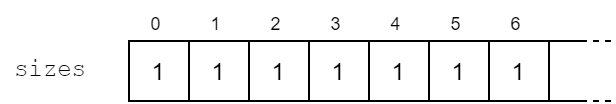
\includegraphics[width=0.7\textwidth]{./images/DisjointSetSizesVector.png}
    	\label{fig:sizes}
    \end{figure}
    
    \item \textbf{parents}: che contiene il nodo padre del nodo attuale etichettato con l'indice corrispondente alla posizione nel vettore dei vertici. Tale vettore dopo l'inizializzazione conterrà dunque, fatta l'assunzione che i vertici siano numerati da 0 a n-1, la posizione attuale nel vettore, in quanto il nodo 0 ha 0 come padre, il nodo 1 ha 1 come suo padre e così via.
    \begin{figure}[h]
    	\caption{Inizializzazione di parents}
    	\centering
    	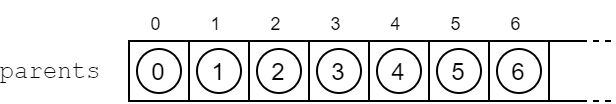
\includegraphics[width=0.7\textwidth]{./images/DisjointSetParentsVector.png}
    	\label{fig:parents}
    \end{figure}
\end{itemize}

Per implementare la classe "DisjointSet" si è scelto di eseguire l'operazione di unione tramite union by size come visto in classe. La seconda versione, ossia "DisjointCompressed" implementa invece l'unione tramite union by rank e path splitting: ogni volta che una find viene chiamata su di un nodo, quest'ultima fa puntare ogni nodo nel percorso nodo-radice a suo nonno, rendendo gli alberi via via sempre meno profondi. La ragione di questa scelta, ossia di aver implementato anche la union by rank con path splitting è per approfondire anche tale soluzione accennata in classe, osservandone il comportamento in termini di velocità di esecuzione. Per avere un'idea di come tale struttura dati è stata implementata con l'uso di questi 2 vettori (sizes e parents) ne riportiamo un esempio in versione union by size nella figura~\ref{fig:disjointset example} e un esempio in versione union by rank e path splitting nella figura~\ref{fig:disjointset path c example}.

\begin{figure}[h]
	\caption{Esempio di unione con DisjointSet}
	\centering
	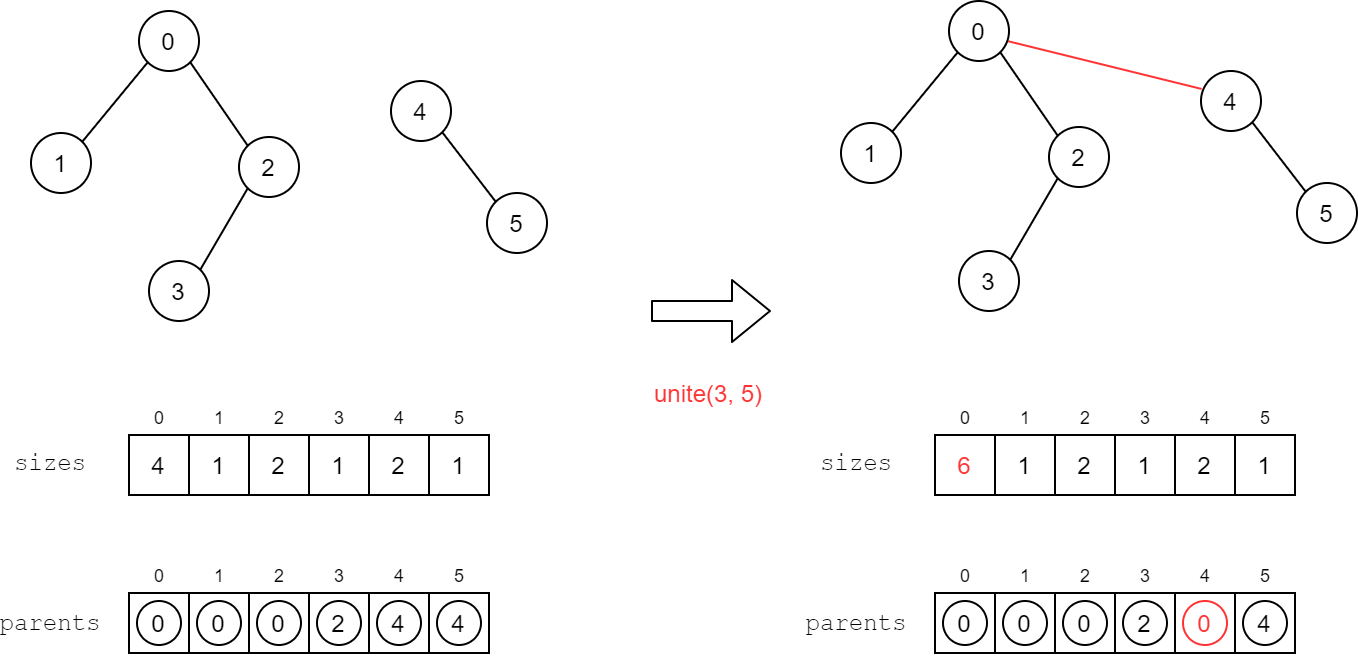
\includegraphics[width=0.7\textwidth]{./images/DisjointSetExample.png}
	\label{fig:disjointset example}
\end{figure}

\begin{figure}[h]
	\caption{Esempio di unione con DisjointCompressed}
	\centering
	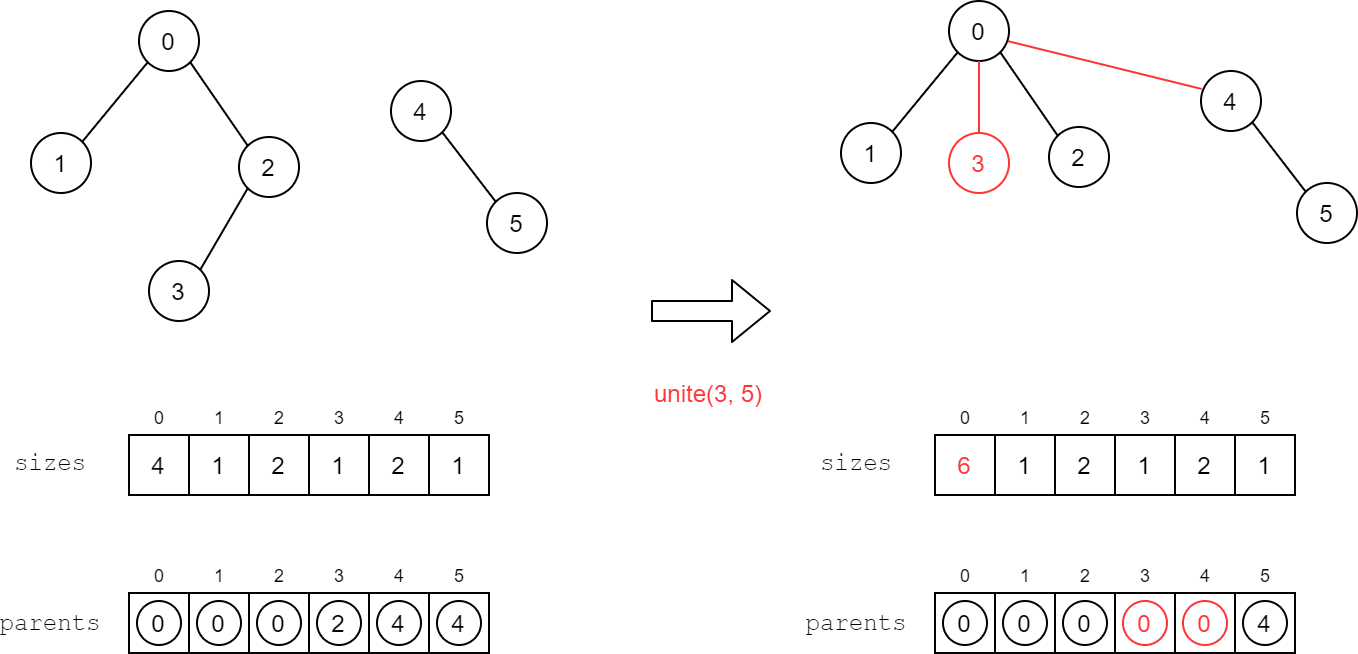
\includegraphics[width=0.7\textwidth]{./images/DisjointSetCompressedExample.png}
	\label{fig:disjointset path c example}
\end{figure}

Infine, per dare una panoramica delle classi che implementano tali strutture dati riportiamo il relativo diagramma di classe, raffigurato in figura ~\ref{fig:DisjointSet Class}.

\begin{figure}[h]
	\caption{Diagramma di classe di DisjointSet}
	\centering
	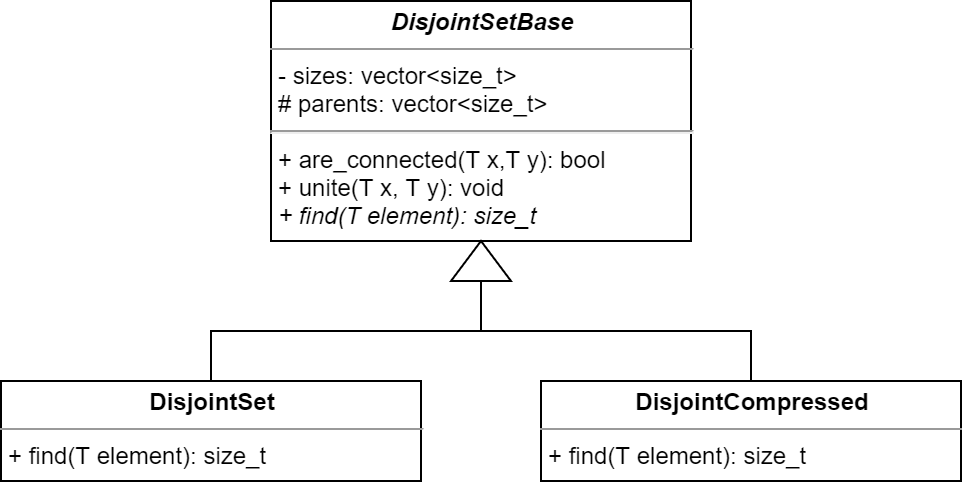
\includegraphics[width=0.7\textwidth]{./images/DisjointSetClass.png}
	\label{fig:DisjointSet Class}
\end{figure}

Come possiamo notare dal diagramma di classe, abbiamo una classe astratta DisjointSetBase che viene implementata dalle classi DisjointSet e DisjointCompressed che implementano i metodi astratti find e union.


